\documentclass[12pt,a4paper,openany,oneside,UTF8]{book}

% 格式控制
%\usepackage[ansi]{inputenc}
%------------------------------------------------------------------------------%
%                                                                              %
%   LaTeX Template for Bachlor Thesis of Northwestern Polytechnical University %
%   Environment Config: TeXLive 2017                                           %
%   * XeTeX 3.14159265-2.6-0.99998 (TeX Live 2017/W32TeX)                      %
%   * BibTeX 0.99d (TeX Live 2017/W32TeX)                                      %
%   Version: 1.5.0.0426                                                        %
%                                                                              %
%------------------------------------------------------------------------------%
%   Copyright by NWPU Metaphysics Office, GPLv3-LICENSE                        %
%------------------------------------------------------------------------------%


%---------------------------------纸张大小设置---------------------------------%
\usepackage{geometry}
% 普通A4格式缩进
\geometry{left=1.25in,right=1.25in,top=1in,bottom=1in}
%------------------------------------------------------------------------------%


%----------------------------------必要库支持----------------------------------%
\usepackage{xcolor} %用于添加颜色支持,可以在文档中使用多种颜色。
\usepackage{tikz} %用于绘制图形和图表,支持各种绘图操作和样式。
\usepackage{layouts} %提供了一系列命令,用于显示和调整LaTeX文档的布局和尺寸。
\usepackage[numbers,sort&compress]{natbib} %用于控制参考文献的格式和样式,支持数字和作者年份两种引用风格。
\usepackage{clrscode} %提供了一些命令和环境,用于排版伪代码和算法描述。
\usepackage{gensymb} %提供了一些数学符号,如度数符号、温度符号等。
\usepackage[final]{pdfpages} %用于将外部PDF文件插入到LaTeX文档中,并控制其显示和排版方式。
%------------------------------------------------------------------------------%


%--------------------------------设置标题与目录--------------------------------%
\usepackage[sf]{titlesec} %将标题设置为无衬线字体
\usepackage{titletoc} %允许您更改目录的字体、格式、缩进和对齐方式等属性
%------------------------------------------------------------------------------%


%--------------------------------添加书签超链接--------------------------------%
\usepackage[unicode=true,colorlinks=false,pdfborder={0 0 0}]{hyperref}
% 在此处修改打开文件操作
\hypersetup{
    bookmarks=true,         % show bookmarks bar?
    pdftoolbar=true,        % show Acrobat’s toolbar?
    pdfmenubar=true,        % show Acrobat’s menu?
    pdffitwindow=true,      % window fit to page when opened
    pdfstartview={FitH},    % fits the width of the page to the window
    pdfnewwindow=true,      % links in new PDF window
}
% 在此处添加文章基础信息
\hypersetup{
    pdftitle={title},
    pdfauthor={author},
    pdfsubject={subject},
    pdfcreator={creator},
    pdfproducer={producer},
    pdfkeywords={key1  key2  key3}
}
%------------------------------------------------------------------------------%


%---------------------------------设置字体大小---------------------------------%
% 行距 1.25
% word 中的行距跟latex中的行距概念不一样。
% word 中,行距 = 单倍行距 x 行距值(1.25),而单倍行距 = 字体大小 x 固定系数(1.297/1.30)
% 默认字体12pt,所以 word 中行距 = 单倍行距 x 1.25 = 12pt x 1.3 x 1.25 = 19.5 pt
% latex 中,默认字体大小 12pt,可以通过设置其 baselineskip = 19.455 pt 来达到word要求的1.25倍行距的效果
% 又因为latex中默认 baselineskip = fontsize x 1.2,所以默认 baselineskip = 12pt x 1.2 = 14.4 pt
% 所以要求的 baselineskip 是默认的 baselineskip 的 19.455/14.4pt = 1.352 倍:
\usepackage{type1cm}
% 字号与行距,统一前缀s(a.k.a size)
%\linespread{1.354}
\newcommand{\sChuhao}{\fontsize{42pt}{63pt}\selectfont}                 % 初号, 1.5倍
\newcommand{\sYihao}{\fontsize{26pt}{36pt}\selectfont}                  % 一号, 1.4倍
\newcommand{\sErhao}{\fontsize{22pt}{28pt}\selectfont}                  % 二号, 1.25倍
\newcommand{\sXiaoer}{\fontsize{18pt}{18pt}\selectfont}                 % 小二, 单倍
\newcommand{\sSanhao}{\fontsize{16pt}{24pt}\selectfont}                 % 三号, 1.5倍
\newcommand{\sXiaosan}{\fontsize{15pt}{22pt}\selectfont}                % 小三, 1.5倍
\newcommand{\sSihao}{\fontsize{14pt}{21pt}\selectfont}                  % 四号, 1.5倍
\newcommand{\sHalfXiaosi}{\fontsize{12.5pt}{16.25pt}\selectfont}        % 半小四, 1.25倍
\newcommand{\sLargeHalfXiaosi}{\fontsize{13pt}{19pt}\selectfont}        % 半小四, 1.5倍
\newcommand{\sXiaosi}{\fontsize{12pt}{14.4pt}\selectfont}               % 小四, 1.25倍
\newcommand{\sLargeWuhao}{\fontsize{11pt}{11pt}\selectfont}             % 大五, 单倍
\newcommand{\sWuhao}{\fontsize{10.5pt}{10.5pt}\selectfont}              % 五号, 单倍
\newcommand{\sXiaowu}{\fontsize{9pt}{9pt}\selectfont}                   % 小五, 单倍
%------------------------------------------------------------------------------%


%---------------------------------设置中文字体---------------------------------%
\usepackage{fontspec}
\usepackage[SlantFont,BoldFont,CJKchecksingle]{xeCJK}
\usepackage{CJKnumb}
% 使用 Adobe 字体
\newcommand\adobeSog{SimSun}
\newcommand\adobeHei{SimHei}
\newcommand\adobeKai{KaiTi}
\newcommand\adobeFag{FangSong}
\newcommand\codeFont{Consolas}

% 设置字体
\defaultfontfeatures{Mapping=tex-text}
\setCJKmainfont[ItalicFont=\adobeKai, BoldFont=\adobeHei]{\adobeSog}
\setCJKsansfont[ItalicFont=\adobeKai, BoldFont=\adobeHei]{\adobeSog}
\setCJKmonofont{\codeFont}
\setmonofont{Times New Roman}
% 设置字体族
\setCJKfamilyfont{song}{\adobeSog}      % 宋体
\setCJKfamilyfont{hei}{\adobeHei}       % 黑体
\setCJKfamilyfont{kai}{\adobeKai}       % 楷体
\setCJKfamilyfont{fang}{\adobeFag}      % 仿宋体
% 用于页眉学校名,特殊字体,powerby https://github.com/ecomfe/fonteditor
\setCJKfamilyfont{nwpu}{nwpuname}
% 新建字体命令,统一前缀f(a.k.a font)
\newcommand{\fSong}{\CJKfamily{song}}
\newcommand{\fHei}{\CJKfamily{hei}}
\newcommand{\fFang}{\CJKfamily{fang}}
\newcommand{\fKai}{\CJKfamily{kai}}
\newcommand{\fNWPU}{\CJKfamily{nwpu}}
%------------------------------------------------------------------------------%


%------------------------------添加插图与表格控制------------------------------%
\usepackage{graphicx}
\usepackage[font=small,labelsep=quad]{caption}
\usepackage{wrapfig}
\usepackage{multirow,makecell}
\usepackage{longtable}
\usepackage{booktabs}
\usepackage{tabularx}
\usepackage{setspace}
\captionsetup[table]{labelfont=bf,textfont=bf}
%------------------------------------------------------------------------------%


%---------------------------------添加列表控制---------------------------------%
\usepackage{enumerate}
\usepackage{enumitem}
%------------------------------------------------------------------------------%


%---------------------------------设置引用格式---------------------------------%
\renewcommand\figureautorefname{图}
\renewcommand\tableautorefname{表}
\renewcommand\equationautorefname{式}
\newcommand\myreference[1]{[\ref{#1}]}
\newcommand\eqrefe[1]{式(\ref{#1})}
% 增加 \ucite 命令使显示的引用为上标形式
\newcommand{\ucite}[1]{$^{\mbox{\scriptsize \cite{#1}}}$}
\renewcommand\arraystretch{1.4}
\renewcommand\theequation{\thesection.\arabic{equation}}
\renewcommand{\thefigure}{\thechapter-\arabic{figure}}
\renewcommand{\thetable}{\thechapter-\arabic{table}}

\usepackage{float}
\setlength{\textfloatsep}{25pt plus 1.0pt minus 2.0pt}
\setlength{\floatsep}{25pt plus 1.0pt minus 2.0pt}
\setlength{\intextsep}{25pt plus 1.0pt minus 2.0pt}

\setlength{\bibsep}{0em} % 设置参考文献条目间的距离
%------------------------------------------------------------------------------%


%--------------------------------设置定理类环境--------------------------------%
\usepackage[amsthm,thmmarks]{ntheorem}
\newtheorem{myexample}{例}
\newtheorem{thm}{定理}
%------------------------------------------------------------------------------%


%--------------------------设置中文段落缩进与正文版式--------------------------%
\XeTeXlinebreaklocale "zh"                      % 使用中文的换行风格
\XeTeXlinebreakskip = 0pt plus 1pt              % 调整换行逻辑的弹性大小
\usepackage{indentfirst}                        % 段首空格设置
\setlength{\parindent}{26pt}                    % 段首空格长度
\setlength{\parskip}{3pt plus 1pt minus 1pt}    % 段落间距
%根据word和latex的行间距转化公式 1.25*1.3/1.2
\renewcommand{\baselinestretch}{1.354}           % 行距
%------------------------------------------------------------------------------%

%---------------------------------设置页眉页脚---------------------------------%
\usepackage{fancyhdr}
\usepackage{fancyref}
%\addtolength{\headsep}{-0.1cm}          %页眉位置
\addtolength{\footskip}{-0.1cm}         %页脚位置
\addtolength{\topmargin}{0cm}
\newcommand{\makeheadrule}{
	\makebox[0pt][l]{\rule[.7\baselineskip]{\headwidth}{0.8pt}}
	\vskip-.8\baselineskip
}
\makeatletter
\renewcommand{\headrule}{%
	{\if@fancyplain\let\headrulewidth\plainheadrulewidth\fi\makeheadrule}}
\pagestyle{fancyplain}
\fancyhf{}
\fancyfoot[C,C]{\sXiaowu~\thepage~} % 设置页脚字体大小
% 后续文字可以自行修改
\chead{\sSanhao\raisebox{0.04cm}%
	{ \fNWPU 西北工业大学} \fSong{{\textbf{本科毕业设计(论文)} }}}
%------------------------------------------------------------------------------%

%----------------------------设置段落标题与目录格式----------------------------%
\setcounter{secnumdepth}{3}
\setcounter{tocdepth}{2}

\newcommand\chapterID[1]{第\CJKnumber{#1}章}
\renewcommand{\chaptername}{第~\CJKnumber{\thechapter}~章}
\renewcommand{\figurename}{图}
\renewcommand{\tablename}{表}
\renewcommand{\bibname}{参考文献}
\renewcommand{\contentsname}{\bfseries 目~录}
\newcommand{\keywords}[1]{\\ \\ \textbf{关键词}:#1}
%\renewcommand{preface/c_abstract}{中文摘要(脑机接口,机器学习,深度学习)}
%\renewcommand{preface/c_abstract}{英文摘要(Brain-Computer\enspace Interface,\enspace Machine\enspace Learning,\enspace Deep\enspace Learning)}



\titleformat{\chapter}[hang]{\normalfont\sSanhao\filcenter\fHei\bf}%
{\sSanhao{\chaptertitlename}}{1em}{\sSanhao}
\titleformat{\section}[hang]{\fHei \bf \sXiaosan}%
{\sXiaosan \thesection}{0.5em}{}{}
\titleformat{\subsection}[hang]{\fHei \bf \sLargeHalfXiaosi}%
{\sLargeHalfXiaosi \thesubsection}{0.5em}{}{}
\titleformat{\subsubsection}[hang]{\fHei \bf}%
{(\arabic{subsubsection})}{0.5em}{}{}   % 小标题式的subsubsection:(4) 标题  % 小标题式的subsubsection:(4) 标题

% 缩小正文中各级标题之间的缩进
\titlespacing{\chapter}{0pt}{15.2pt}{14.4pt}
\titlespacing{\section}{0pt}{-3pt}{2pt}
\titlespacing{\subsection}{0pt}{-2.5pt}{-2.5pt}
\titlespacing{\subsubsection}{0pt}{0.25em}{0pt}

% 定义目录中各级标题之间的格式以及缩进
\dottedcontents{section}[1.16cm]{}{1.8em}{5pt}
\dottedcontents{subsection}[2.00cm]{}{2.7em}{5pt}
\dottedcontents{subsubsection}[2.86cm]{}{3.4em}{5pt}
\titlecontents{chapter}[0pt]{\fHei\vspace{0.5em}}%
{\contentsmargin{0pt}\fHei\makebox[0pt][l]{\chapterID{\thecontentslabel}}\hspace{3.8em}}%
{\contentsmargin{0pt}\fHei}%
{\titlerule*[.5pc]{.}\contentspage}[\vspace{0em}]
%------------------------------------------------------------------------------%





%----------------------------------其他补充设置--------------------------------%
% 重置列表环境的间隔
% \let\orig@Itemize =\itemize
% \let\orig@Enumerate =\enumerate
% \let\orig@Description =\description

% \def\Myspacing{
%     \itemsep=1.5ex \topsep=-0.5ex \partopsep=0pt \parskip=0pt \parsep=0.5ex
% }

% \def\newitemsep{
%     \renewenvironment{itemize}{\orig@Itemize\Myspacing}{\endlist}
%     \renewenvironment{enumerate}{\orig@Enumerate\Myspacing}{\endlist}
%     \renewenvironment{description}{\orig@Description\Myspacing}{\endlist}
% }

% \def\olditemsep{
%     \renewenvironment{itemize}{\orig@Itemize}{\endlist}
%     \renewenvironment{enumerate}{\orig@Enumerate}{\endlist}
%     \renewenvironment{description}{\orig@Description}{\endlist}
% }

% \newitemsep
% 下划线
\newcommand\dlmu@underline[2][5cm]%
{\hskip1pt\underline{\hb@xt@ #1{\hss#2\hss}}\hskip3pt}
\let\coverunderline\dlmu@underline
%------------------------------------------------------------------------------%


%----------------------------------添加代码控制--------------------------------%
\usepackage{listings}
\lstset{
    basicstyle=\footnotesize\ttfamily,
    numbers=left,
    numberstyle=\tiny,
    numbersep=5pt,
    tabsize=4,
    extendedchars=true,
    breaklines=true,
    keywordstyle=\color{blue}\bfseries,
    numberstyle=\color{purple},
    commentstyle=\color[rgb]{0, 0.4, 0}\bfseries,
    stringstyle=\color{violet}\ttfamily\bfseries,
    rulesepcolor=\color{red!20!green!20!blue!20},
    showspaces=false,
    showtabs=false,
    frame=shadowbox,
    framexrightmargin=5pt,
    framexbottommargin=4pt,
    showstringspaces=false,
    escapeinside=`', %逃逸字符(1左面的键),用于显示中文
}
\renewcommand{\lstlistingname}{CODE}
\lstloadlanguages{% Check Dokumentation for further languages, page 12
    Pascal, C++, Java, Ruby, Python, Matlab, R, Haskell
}
%------------------------------------------------------------------------------%

\endinput
% 这是简单的 thesis(book) 的导言区设置,不能单独编译。

% 非格式控制插件
% \usepackage{math-symbols}
% \usepackage{plug-ins/math-symbols}
% Longitudinal coefficients
\newcommand\CL{{C_L}}
\newcommand\CLz{{C_{L_0}}}
\newcommand\CLa{{C_{L_\alpha}}}
\newcommand\CLq{{C_{L_q}}}
\newcommand\CLde{{C_{L_{\delta_e}}}}
\newcommand\CD{{C_D}}
\newcommand\CDz{{C_{D_0}}}
\newcommand\CDa{{C_{D_\alpha}}}
\newcommand\CDq{{C_{D_q}}}
\newcommand\CDde{{C_{D_{\delta_e}}}}
\newcommand\Cm{{C_m}}
\newcommand\Cmz{{C_{m_0}}}
\newcommand\Cma{{C_{m_\alpha}}}
\newcommand\Cmq{C_{m_q}}
\newcommand\Cmde{C_{m_{\delta_e}}}
\newcommand\Cmcl{{C_{m_{C_L}}}}

% Lateral coefficients
\newcommand\CY{C_Y}
\newcommand\CYz{C_{Y_0}}
\newcommand\CYb{C_{Y_\beta}}
\newcommand\CYp{C_{Y_p}}
\newcommand\CYr{C_{Y_r}}
\newcommand\CYda{C_{Y_{\delta_a}}}
\newcommand\CYdr{C_{Y_{\delta_r}}}
\newcommand\Cl{C_l}
\newcommand\Clz{C_{l_0}}
\newcommand\Clb{C_{l_\beta}}
\newcommand\Clp{C_{l_p}}
\newcommand\Clr{C_{l_r}}
\newcommand\Clda{C_{l_{\delta_a}}}
\newcommand\Cldr{C_{l_{\delta_r}}}
\newcommand\Cn{C_n}
\newcommand\Cnz{C_{n_0}}
\newcommand\Cnb{C_{n_\beta}}
\newcommand\Cnp{C_{n_p}}
\newcommand\Cnr{C_{n_r}}
\newcommand\Cnda{C_{n_{\delta_a}}}
\newcommand\Cndr{C_{n_{\delta_r}}}

% Controls
\newcommand\da{{\delta_a}}
\newcommand\de{{\delta_e}}
\newcommand\dr{{\delta_r}}
\newcommand\dt{{\delta_t}}

% factor
\newcommand\q{{\frac{1}{2} \rho V^2}}       % 1/2 rho V^2
\newcommand\qs{{\frac{1}{2} \rho V^2 S}}    % 1/2 rho V^2

% others
\newcommand\CW{{C_W}}

\endinput

% 插图目录
\graphicspath{{figures/}}

%核心就是下面三段代码
\usepackage{amsmath}
\usepackage{float}
\numberwithin{equation}{section}%公式按章节编号
\numberwithin{figure}{section}%图表按章节编号
%\setCJKmainfont[AutoFakeBold=2.7]{\Sog}
\begin{document}


\sloppy

\pagenumbering{Roman}

% 封皮
\frontmatter
% 本科毕业设计论文模板
% 封皮
\begin{titlepage}
    \voffset 2.7cm
    \begin{center}
        \begin{center}
            \begin{minipage}[c]{2.64cm}
                \centering
                \resizebox{!}{0.9cm}{ \parbox{0.54cm}{ \begin{tikzpicture}
    \draw[line width=0.10cm] (0, 0) circle (2.0cm);
    % \fill[gray!15] (0, 0) -- (1.3cm,0cm) arc (0:230:1.3cm) -- cycle;
    % \fill[gray!15] (0, 0) -- (1.3cm,0cm) arc (0:-50:1.3cm) -- cycle;
    \foreach \t in {-50, -40, -30, -20, -10, 0, 10, 20, 30, 40, 50, 60, 70, 80, 90, 100, 110, 120, 130, 140, 150, 160, 170, 180, 190, 200, 210, 220, 230}
    {
        \foreach \p/\d in {0/0.01cm, 5/-0.01cm}
        {
            \foreach \r in {1.27cm, 1.17cm, 1.07cm, 0.97cm}
            {
                \fill (\t + \p: \r + \d) circle (0.01cm);
            }
        }
    };
    \draw[line width=0.03cm] (0, 0) circle (1.32cm);
    \fill[white] (0, 0) circle (0.9cm);
    \draw[line width=0.05cm] (0, 0) circle (0.9cm);
    \fill[black] (-0.50, -0.73) .. controls (-0.35, -0.81) ..
        (-0.2, -0.80) .. controls (0.15, -0.70) and (0.20, -0.60) .. 
        (0.35, -0.35) .. controls (0.42, -0.24) and (0.60, -0.26) ..
        (0.60, -0.40) .. controls (0.58, -0.50) and (0.49, -0.50) ..
        (0.45, -0.45) .. controls (0.40, -0.68) and (0.75, -0.70) ..
        (0.90, 0.00) arc (360:250:0.9cm);
    \fill (-0.40, -0.40)--(-1.33, -0.40)--(1.00, 1.10)--cycle;
    \fill (-0.37, -0.43)--(-0.20, -0.80)--(1.01, 1.05)--cycle;
    
    \foreach \x/\txt in {0/N, 1/O, 2/R, 3/T, 4/H, 5/W, 6/E, 7/S, 8/T, 9/E, 10/R, 11/N, 12/~, 13/P, 14/O, 15/L, 16/Y, 17/T, 18/E, 19/C, 20/H, 21/N, 22/I, 23/C, 24/A, 25/L, 26/~, 27/U, 28/N, 29/I, 30/V, 31/E, 32/R, 33/S, 34/I, 35/T, 36/Y}
    {
        \node[scale=0.7, rotate=\x*-6.50-245] at (207+\x*-6.50:1.6cm) {\txt};
    };

    \foreach \x/\txt in {0/西, 1/北, 2/工, 3/业, 4/大, 5/学}
    {
        \node[scale=1.25, rotate=\x*18-50] at (225+\x*18:1.65cm) {\fNWPU\txt};
    };

    \foreach \x/\txt in {0/1, 1/9, 2/3, 3/8}
    {
        \node[scale=1, rotate=\x*18-25] at (\x*18-115:1.1cm) {\bfseries\txt};
    };
\end{tikzpicture}

\endinput
% 这是西北工业大学校徽文件,不能单独编译。 } }
                \end{minipage}
                \hskip 0.8cm
                \begin{minipage}[c]{8cm}
                \fontsize{33}{33}\fNWPU 西北工业大学
            \end{minipage}
        \end{center}
        \vskip 0.7cm
        \sChuhao\fSong {\bfseries 本科毕业设计(论文)}
        \vskip 5cm
        {
        \sSanhao\fHei 题~~目 \hspace{0.2cm}\coverunderline[12.5cm]{基于人工智能的多用途脑机接口脑电图工具箱开发}
        }
        \vskip 2cm
        {
            \sSihao\fSong 专业名称\coverunderline[5.5cm]{XXX}
            \vskip 0.7cm
            \sSihao\fSong 学生姓名\coverunderline[5.5cm]{XXX}
            \vskip 0.7cm
            \sSihao\fSong 指导教师\coverunderline[5.5cm]{XXX}
            \vskip 0.7cm
            \sSihao\fSong 毕业时间\coverunderline[5.5cm]{2023年7月}
            \vfill
        }
    \end{center}
\end{titlepage}
\fSong \normalsize

\endinput
% 这是封面排版文件,不能单独编译。
%\clearpage
%\thispagestyle{empty}\textbf{}
%\phantom{s}
%\clearpage
%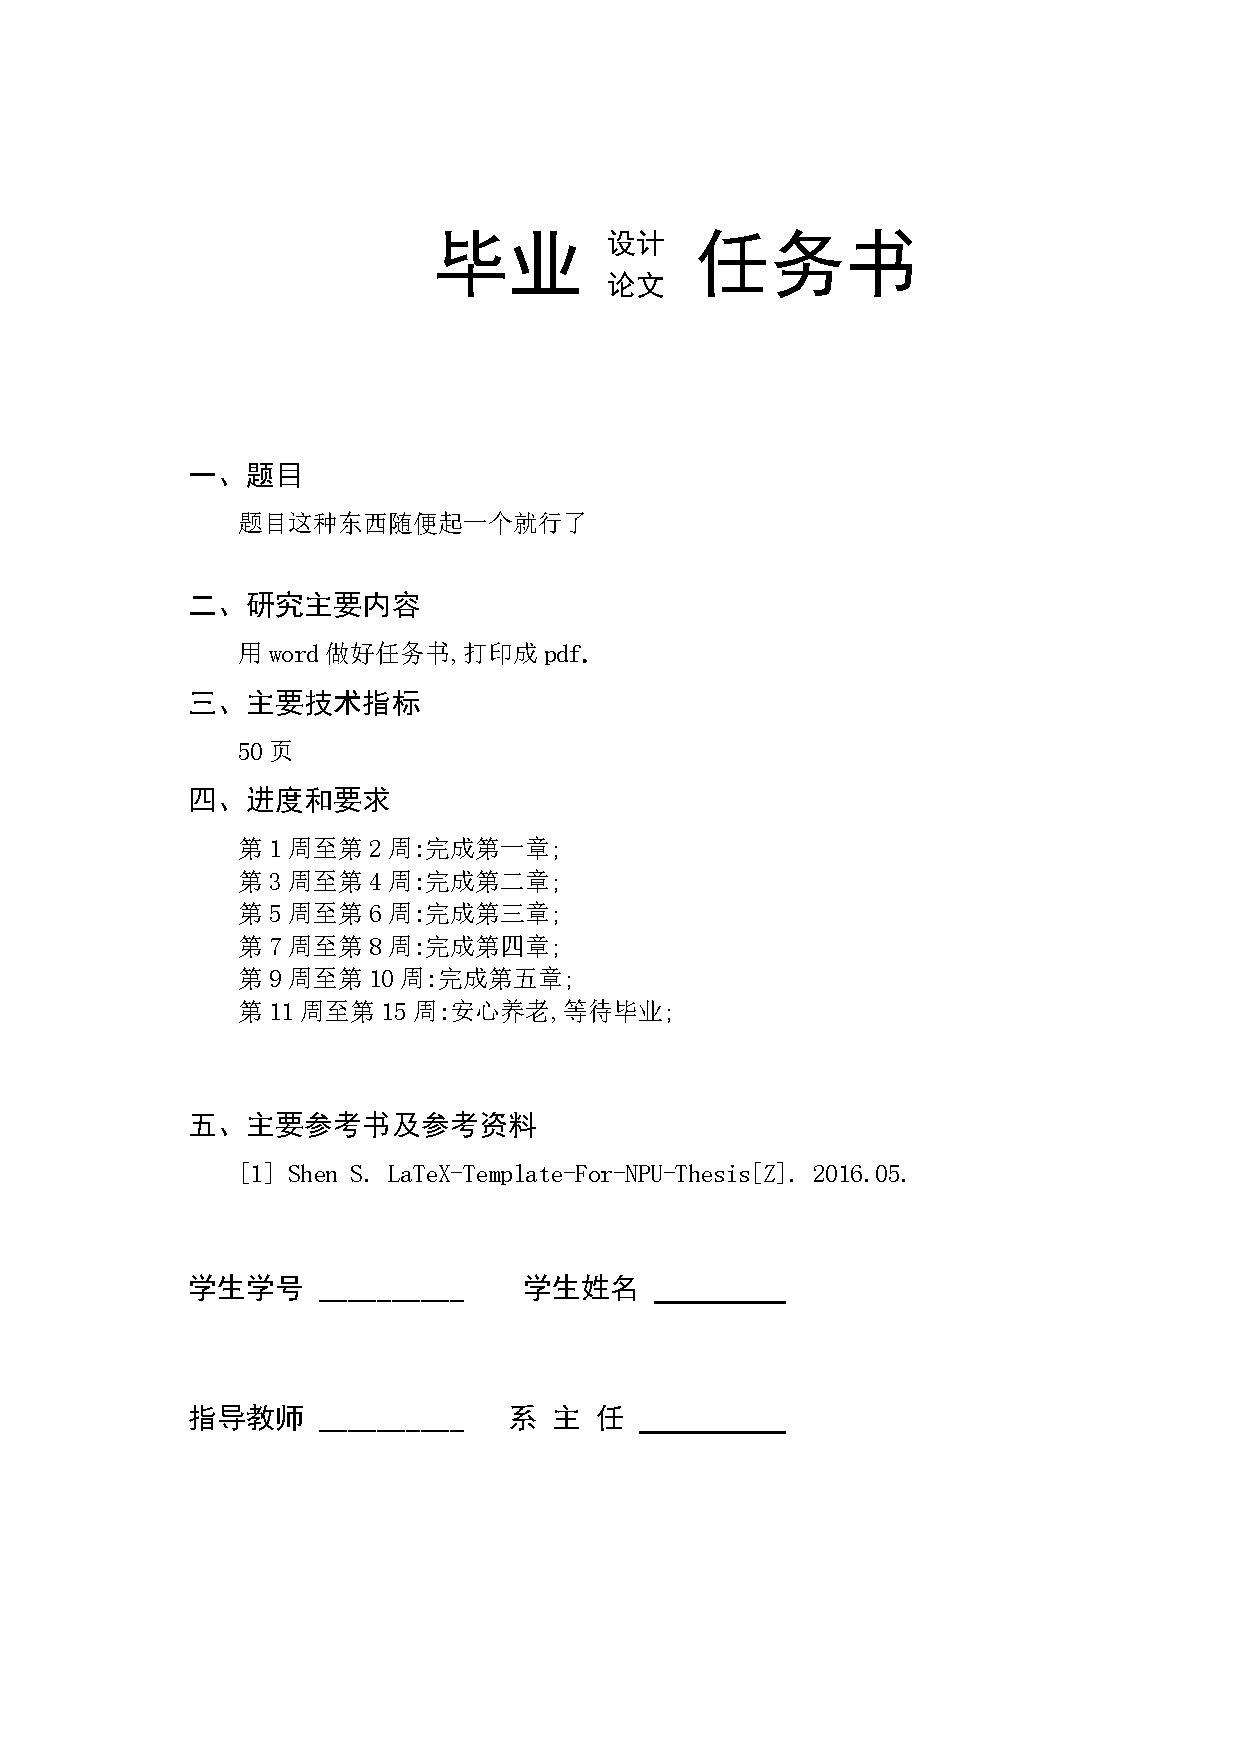
\includepdf{preface/tasklist.pdf}
%\newpage
%\clearpage
%\thispagestyle{empty}
%\phantom{s}
%\clearpage

\setcounter{page}{1}
\pagenumbering{Roman}


%根据word和latex的中文行间距转化公式 1.25*1.15/1.2
\renewcommand{\baselinestretch}{1.345}

% 中文摘要
\renewcommand{\baselinestretch}{1.345}
\fontsize{12pt}{14.4pt}\selectfont

%\renewcommand{\abstractname}{中文摘要}
\chapter*{摘~要}

\markboth{中~文~摘~要}{中~文~摘~要}

这里填写摘要

综上, 本文主要做的工作有:
\vspace{-10pt}
\begin{enumerate}
	\item 本文首先
	\item 本文介绍
	\item 本文通过
\end{enumerate}
\vspace{-10pt}

\vspace{1em}
\noindent {\fHei 关键词:}机器学习,深度学习

\clearpage
\endinput

% 英文摘要
\setmainfont{Times New Roman}
\renewcommand{\baselinestretch}{1.2}
\fontsize{12pt}{14.4pt}\selectfont
%\renewcommand{\abstractname}{Abstract}
\titleformat{\chapter}[hang]{\normalfont\sSanhao\filcenter}%
{\sSanhao{\chaptertitlename}}{1em}{\sSanhao}
\chapter*{ABSTRACT}

\markboth{英~文~摘~要}{英~文~摘~要}

This is ABSTRACT



\vspace{-12pt}
\begin{enumerate} \setlength{\itemsep}{0pt}
    \item This paper analyzes 
    \item This article demonstrates 
\end{enumerate}
\vspace{-12pt}


\vspace{1em}
\noindent \textbf{KEY\!\, WORDS:}\enspace Interface,\enspace Machine\enspace Learning,\enspace Deep\enspace Learning

\clearpage
\endinput

\renewcommand{\baselinestretch}{1.354}
\fontsize{12pt}{12pt}\selectfont
\phantomsection
%\addcontentsline{toc}*{\fHei}
\tableofcontents
\clearpage

\mainmatter
\sHalfXiaosi\fSong

% 正文内容
\titleformat{\chapter}[hang]{\normalfont\sSanhao\filcenter\fHei\bf}%
{\sSanhao{\chaptertitlename}}{1em}{\sSanhao}
%根据word和latex的中文行间距转化公式 1.25*1.3/1.2
\renewcommand{\baselinestretch}{1.345}
\fontsize{12pt}{14.4pt}\selectfont
\chapter{绪论}
\section{研究目的与意义}
绪论
\section{国内外发展状况}
\subsection{MATLAB工具箱的发展现状}

1234
\subsection{脑机接口概述与现状}
1234 引用\ucite{reference3}\ucite{reference20}。

引用见参考文献的bib格式\ucite{reference5}。

\section{研究内容}

图像引用格式
\begin{figure}[ht]
	\centering
	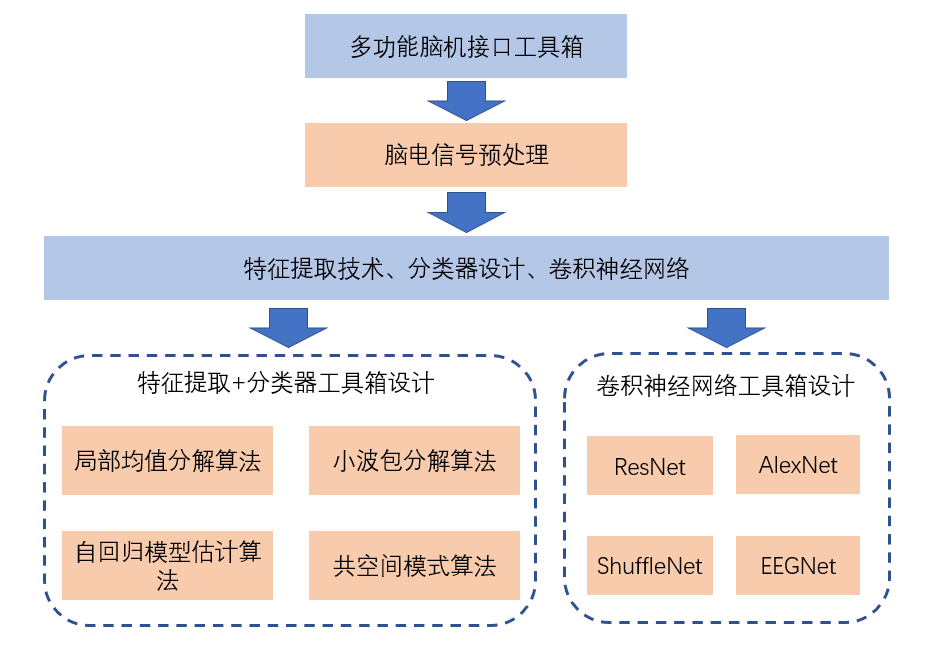
\includegraphics[scale=0.65]{figures/研究内容.png}
	\caption{
		研究内容
	}
	\label{研究内容}
\end{figure}
列表格式
\begin{enumerate}
\item 5.。
\item 4.。
\item 3.。
\item 2.。
\item 1.。
\end{enumerate}

\endinput


%根据word和latex的中文行间距转化公式 1.25*1.3/1.2
\renewcommand{\baselinestretch}{1.345}
\fontsize{12pt}{14.4pt}\selectfont
\chapter{功能分析}
第二章这里写
\section{总体设计思想}

这里写2.1

\endinput

%根据word和latex的中文行间距转化公式 1.25*1.3/1.2
\renewcommand{\baselinestretch}{1.345}
\fontsize{12pt}{14.4pt}\selectfont
\chapter{从图像预处理到分类器设计}
演示一下公式编写
数学表达式如(\ref{equ1}):
\begin{equation}
y[n] = \sum_{k =0}^{N-1}\omega[k] \times x[n-k] 
\label{equ1}
\end{equation}

其中$N-1$表示FIR滤波器的阶数,$\omega$是窗函数。常用的窗函数有矩形窗函数、Hamming窗函数、Hanning窗函数和Blackman函数,本文设计的工具箱使用的Hamming窗函数。


\endinput
% 参考文献设置
\clearpage
\phantomsection
\addcontentsline{toc}{chapter}{\fHei 参考文献}
\sSihao 
% npu专用

\bibliographystyle{settings/nputhesis}


% 参考文献位置
\begin{spacing}{1.345} 
\bibliography{references/reference}
  \end{spacing} 

% 附录
\backmatter
\renewcommand{\baselinestretch}{1.345}
\fontsize{12pt}{14.4pt}\selectfont
\phantomsection
\chapter*{致~~~~谢}
\addcontentsline{toc}{chapter}{\fHei 致谢}

写致谢

\clearpage
\endinput

%根据word和latex的中文行间距转化公式 1.25*1.3/1.2
\renewcommand{\baselinestretch}{1.345}
\fontsize{12pt}{14.4pt}\selectfont
\phantomsection
\chapter*{毕业设计小结}
\addcontentsline{toc}{chapter}{\fHei 毕业设计小结}

毕业小结写一下

\clearpage
\endinput

%根据word和latex的中文行间距转化公式 1.25*1.3/1.2
\renewcommand{\baselinestretch}{1.345}
\fontsize{12pt}{14.4pt}\selectfont
\phantomsection
\chapter*{附~~~~录}

\addcontentsline{toc}{chapter}{\fHei 附录}
写一下附录,我这里表格就不改了大家可以参考写自己的表格
\begin{table}[!ht]
	\centering
	\caption{脑机接口工具箱接口对照表}\label{label2}
	\setlength{\tabcolsep}{5mm}
	{
		\begin{tabular}{|c|c|c|}
			\hline
			模块                     & 函数              & 函数功能                                                      \\ \hline
			\multirow{4}{*}{图像预处理} & pop\_eegfiltnew & 对数据进行滤波                                                   \\ \cline{2-3} 
			& pop\_epoch      & 对二维数据根据事件信息进行分段                                           \\ \cline{2-3} 
			& pop\_rmbase     & 对分段数据基线校正                                                 \\ \cline{2-3} 
			& pop\_resample   & 对分段数据及进行降采样                                               \\ \hline
			\multirow{4}{*}{特征提取}  & LMD             & 对分段数据提取LMD特征                                              \\ \cline{2-3} 
			& WPD             & 对分段数据提取WPD特征                                              \\ \cline{2-3} 
			& AR              & 对分段数据提取AR特征                                               \\ \cline{2-3} 
			& CSP             & 对分段数据提取CSP特征投影矩阵                                          \\ \hline
			\multirow{2}{*}{分类器}   & SVM             & 训练支持向量机 \\ \cline{2-3} 
			& multSVM         & 训练基于一对多的多分类支持向量机                          \\ \hline
			\multirow{7}{*}{深度学习}  & myResNet18      & 训练ResNet网络                                                \\ \cline{2-3} 
			& myResNet50      & 训练ResNet50网络                                              \\ \cline{2-3} 
			& myshuffleNet    & 训练shuffleNet网络                                            \\ \cline{2-3} 
			& mySqeezeNet     & 训练SqueezeNet网络                                            \\ \cline{2-3} 
			& myAlexNet       & 训练AlexNet网络                                               \\ \cline{2-3} 
			& myEEGNet        & 训练EEGNet网络                                                \\ \cline{2-3} 
			& mySingleCNN     & 训练SingleCNN网络                                             \\ \hline
			\multirow{2}{*}{其他}    & getresult       & 生成相关评估数据,并绘制混淆矩阵图                                         \\ \cline{2-3} 
			& one\_hot        & 根据多标签数据生成one\_hot数据标签集                                    \\ \hline
		\end{tabular}
	}
\end{table}

\clearpage
\endinput

\clearpage
\end{document}


